\documentclass{article}

\usepackage[utf8]{inputenc}
\usepackage[letterpaper, total={6in, 9in}]{geometry}
\usepackage{amsmath}
\usepackage{natbib}
\usepackage{wrapfig}
\usepackage{graphicx}
\usepackage{amssymb}
\usepackage{tikz}
\graphicspath{ {./geo3/} }

\title{Geometry 3 - Miscellaneous}
\author{TSS Math Club}
\date{Nov 2022}

\begin{document}
\large

\maketitle

\section{Pythagorean Theorem}

\begin{wrapfigure}{R}{0.4\textwidth} %this figure will be at the right
    \centering
    
    \tikzset{every picture/.style={line width=0.75pt}} %set default line width to 0.75pt        

    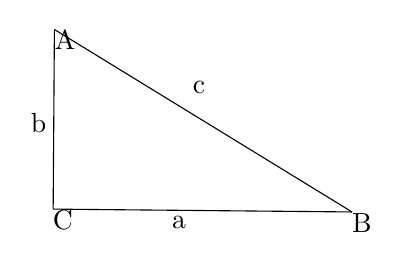
\begin{tikzpicture}[x=0.75pt,y=0.75pt,yscale=-1,xscale=1]
    %uncomment if require: \path (0,300); %set diagram left start at 0, and has height of 300

    %Straight Lines [id:da7810882093328524] 
    \draw    (99.61,122) -- (99.01,208.55) ;
    %Straight Lines [id:da0001872892319363384] 
    \draw    (99.61,122) -- (243.01,209.92) ;
    %Straight Lines [id:da14609712871080904] 
    \draw    (99.01,208.55) -- (243.01,209.92) ;

    % Text Node
    \draw (98.41,121.4) node [anchor=north west][inner sep=0.75pt]   [align=left] {A};
    % Text Node
    \draw (241.81,209.32) node [anchor=north west][inner sep=0.75pt]   [align=left] {B};
    % Text Node
    \draw (97.61,207.94) node [anchor=north west][inner sep=0.75pt]   [align=left] {C};
    % Text Node
    \draw (165,146) node [anchor=north west][inner sep=0.75pt]   [align=left] {c};
    % Text Node
    \draw (155,211) node [anchor=north west][inner sep=0.75pt]   [align=left] {a};
    % Text Node
    \draw (87,161) node [anchor=north west][inner sep=0.75pt]   [align=left] {b};


    \end{tikzpicture}

\end{wrapfigure}

In a right-triangle, 
$$a^2+b^2=c^2$$
where a and b are two sides and c is the hypotenuse.

\subsection{Proof}


\tikzset{every picture/.style={line width=0.75pt}} %set default line width to 0.75pt        

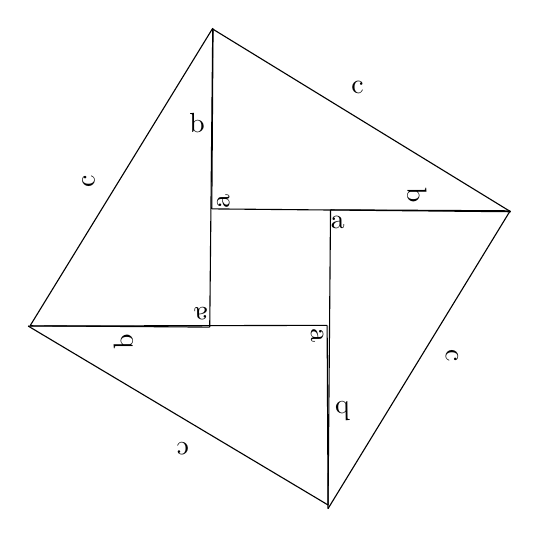
\begin{tikzpicture}[x=0.75pt,y=0.75pt,yscale=-1,xscale=1]
%uncomment if require: \path (0,389); %set diagram left start at 0, and has height of 389

%Straight Lines [id:da7810882093328524] 
\draw    (132.61,28) -- (132.01,114.55) ;
%Straight Lines [id:da0001872892319363384] 
\draw    (132.61,28) -- (276.01,115.92) ;
%Straight Lines [id:da14609712871080904] 
\draw    (132.01,114.55) -- (276.01,115.92) ;
%Straight Lines [id:da17225998918083474] 
\draw    (44.47,170.87) -- (131.02,171.51) ;
%Straight Lines [id:da9772684531569544] 
\draw    (44.47,170.87) -- (132.47,27.51) ;
%Straight Lines [id:da0643086164519977] 
\draw    (131.02,171.51) -- (132.47,27.51) ;
%Straight Lines [id:da6587126862106818] 
\draw    (188.03,257.21) -- (187.58,170.66) ;
%Straight Lines [id:da6536516511809205] 
\draw    (188.03,257.21) -- (43.57,171.02) ;
%Straight Lines [id:da004505283584124831] 
\draw    (187.58,170.66) -- (43.57,171.02) ;
%Straight Lines [id:da0382305085022161] 
\draw    (275.77,115.49) -- (189.22,114.99) ;
%Straight Lines [id:da11791847320342042] 
\draw    (275.77,115.49) -- (188,258.99) ;
%Straight Lines [id:da5759579560679966] 
\draw    (189.22,114.99) -- (188,258.99) ;

% Text Node
\draw (198,52) node [anchor=north west][inner sep=0.75pt]   [align=left] {c};
% Text Node
\draw (188,117) node [anchor=north west][inner sep=0.75pt]   [align=left] {a};
% Text Node
\draw (120,67) node [anchor=north west][inner sep=0.75pt]   [align=left] {b};
% Text Node
\draw (68.51,105.49) node [anchor=north west][inner sep=0.75pt]  [rotate=-270.03] [align=left] {c};
% Text Node
\draw (133.5,115.53) node [anchor=north west][inner sep=0.75pt]  [rotate=-270.03] [align=left] {a};
% Text Node
\draw (83.47,183.5) node [anchor=north west][inner sep=0.75pt]  [rotate=-270.03] [align=left] {b};
% Text Node
\draw (122.35,234) node [anchor=north west][inner sep=0.75pt]  [rotate=-179.31] [align=left] {c};
% Text Node
\draw (131.57,168.88) node [anchor=north west][inner sep=0.75pt]  [rotate=-179.31] [align=left] {a};
% Text Node
\draw (200.16,218.06) node [anchor=north west][inner sep=0.75pt]  [rotate=-179.31] [align=left] {b};
% Text Node
\draw (251.84,180.91) node [anchor=north west][inner sep=0.75pt]  [rotate=-89.94] [align=left] {c};
% Text Node
\draw (186.83,170.98) node [anchor=north west][inner sep=0.75pt]  [rotate=-89.94] [align=left] {a};
% Text Node
\draw (236.76,102.93) node [anchor=north west][inner sep=0.75pt]  [rotate=-89.94] [align=left] {b};


\end{tikzpicture}


\pagebreak

\section{Trigonometry}

\subsection{Definitions}

Sine or $\sin(\theta)$ :
\\ \\
Cosine or $\cos(\theta)$ :
\\ \\
Tangent or $\tan(\theta)$ :

\subsection{Pythagorean Theorem}
$$\sin^2 (\theta)+\cos^2 (\theta)=1$$

\subsection{Triangle Area Formula with Sine}

$$S=\frac{ab\sin C}{2}$$

\subsubsection{Proof}
\vspace{40px}


\subsection{Law of Sines}

$$\frac{a}{\sin A}=\frac{b}{\sin B}=\frac{c}{\sin C}=2R=d$$

\subsubsection{Proof}
\vspace{100px}

\subsection{Law of Cosines}
$$c^2=a^2+b^2-2 a b \cos C $$

\subsubsection{Proof}

\pagebreak

\subsection{Problem}
\subsubsection{Heron's Formula}
$$S= \sqrt {s (s-a) (s-b) (s-c)}, s=\frac{a+b+c}{2}$$


\vspace{200px}


\subsubsection{Problem}
Given AB=3,BD=1,DC=3,AC=2. Find AD.




\tikzset{every picture/.style={line width=0.75pt}} %set default line width to 0.75pt        

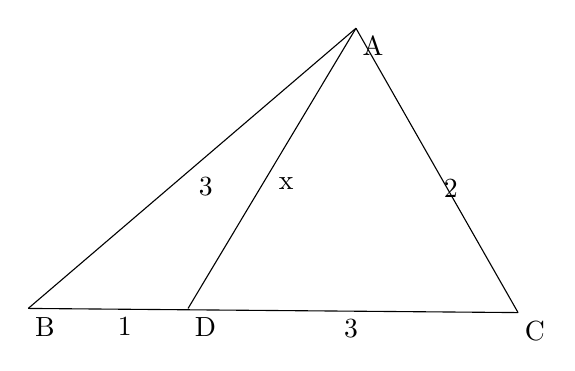
\begin{tikzpicture}[x=0.75pt,y=0.75pt,yscale=-1,xscale=1]
%uncomment if require: \path (0,389); %set diagram left start at 0, and has height of 389

%Straight Lines [id:da28332928208796315] 
\draw    (128.06,259.03) -- (364.06,261.03) ;
%Straight Lines [id:da647118791580753] 
\draw    (285.96,124.03) -- (128.06,259.03) ;
%Straight Lines [id:da4424909815278173] 
\draw    (285.96,124.03) -- (364.06,261.03) ;
%Straight Lines [id:da11044244004039627] 
\draw    (285.96,124.03) -- (205.06,259.03) ;

% Text Node
\draw (287.96,127.03) node [anchor=north west][inner sep=0.75pt]   [align=left] {A};
% Text Node
\draw (130.06,262.03) node [anchor=north west][inner sep=0.75pt]   [align=left] {B};
% Text Node
\draw (366.06,264.03) node [anchor=north west][inner sep=0.75pt]   [align=left] {C};
% Text Node
\draw (207.06,262.03) node [anchor=north west][inner sep=0.75pt]   [align=left] {D};
% Text Node
\draw (209.01,194.53) node [anchor=north west][inner sep=0.75pt]   [align=left] {3};
% Text Node
\draw (170,262) node [anchor=north west][inner sep=0.75pt]   [align=left] {1};
% Text Node
\draw (279,263) node [anchor=north west][inner sep=0.75pt]   [align=left] {3};
% Text Node
\draw (327.01,195.53) node [anchor=north west][inner sep=0.75pt]   [align=left] {2};
% Text Node
\draw (247.51,194.53) node [anchor=north west][inner sep=0.75pt]   [align=left] {x};


\end{tikzpicture}

\pagebreak

\subsubsection{Problem, Euclid 2022 Q8 b)}
Consider the following statement:
\begin{quote}
There is a triangle that is not equilateral whose side lengths form
a geometric sequence, and the measures of whose angles form an
arithmetic sequence.
\end{quote}
Show that this statement is true by finding such a triangle or prove that it is false
by demonstrating that there cannot be such a triangle.


\pagebreak

\section{Transversals}

\subsection{Directed Segments}
Definition
\vspace{30px}

\subsection{Stewart's Theorem}
If A,B,C collinear and P is any other point, then
$$PA^2\cdot BC+PB^2\cdot CA+PC^2\cdot AB+BC \cdot CA \cdot AB =0$$ 



\tikzset{every picture/.style={line width=0.75pt}} %set default line width to 0.75pt        

\begin{tikzpicture}[x=0.75pt,y=0.75pt,yscale=-1,xscale=1]
%uncomment if require: \path (0,300); %set diagram left start at 0, and has height of 300

%Straight Lines [id:da5905118684092199] 
\draw    (52.91,172.03) -- (504.91,177.03) ;
%Straight Lines [id:da9618382085114188] 
\draw    (124,172) -- (233.91,52.03) ;
%Straight Lines [id:da976888364842182] 
\draw    (233.91,52.03) -- (205.91,174.03) ;
%Straight Lines [id:da13878852480396842] 
\draw    (233.91,52.03) -- (442.91,176.03) ;

% Text Node
\draw (126,175) node [anchor=north west][inner sep=0.75pt]   [align=left] {A};
% Text Node
\draw (207.91,177.03) node [anchor=north west][inner sep=0.75pt]   [align=left] {B};
% Text Node
\draw (444.91,179.03) node [anchor=north west][inner sep=0.75pt]   [align=left] {C};
% Text Node
\draw (235.91,55.03) node [anchor=north west][inner sep=0.75pt]   [align=left] {P};


\end{tikzpicture}


\pagebreak

\subsection{Menelaus' Theorem}

Suppose we have a triangle ABC, and a transversal line that crosses BC, AC, and AB at points D, E, and F respectively, with D, E, and F distinct from A, B, and C, then

$$\frac{AF}{FB}\cdot \frac{BD}{DC} \cdot \frac{CE}{EA}=-1$$



\tikzset{every picture/.style={line width=0.75pt}} %set default line width to 0.75pt        

\begin{tikzpicture}[x=0.75pt,y=0.75pt,yscale=-1,xscale=1]
%uncomment if require: \path (0,300); %set diagram left start at 0, and has height of 300

%Straight Lines [id:da01433999833467725] 
\draw    (131,196) -- (522.91,204.03) ;
%Straight Lines [id:da17936156092470434] 
\draw    (172.91,51.03) -- (310.91,200.03) ;
%Straight Lines [id:da243500674973548] 
\draw    (172.91,51.03) -- (131,196) ;
%Straight Lines [id:da01379280330610988] 
\draw    (110,95) -- (535.91,260.03) ;

% Text Node
\draw (174.91,54.03) node [anchor=north west][inner sep=0.75pt]   [align=left] {A};
% Text Node
\draw (133,199) node [anchor=north west][inner sep=0.75pt]   [align=left] {B};
% Text Node
\draw (312.91,203.03) node [anchor=north west][inner sep=0.75pt]   [align=left] {C};
% Text Node
\draw (381,202) node [anchor=north west][inner sep=0.75pt]   [align=left] {D};
% Text Node
\draw (272.91,160.03) node [anchor=north west][inner sep=0.75pt]   [align=left] {E};
% Text Node
\draw (155,115) node [anchor=north west][inner sep=0.75pt]   [align=left] {F};


\end{tikzpicture}

\vspace{200px}

\subsection{Menelaus' Inverse Theorem}

Suppose we have a triangle ABC with D on BC, E on AC, F on AB, such that,
$$\frac{AF}{FB}\cdot \frac{BD}{DC} \cdot \frac{CE}{EA}=-1$$
then D,E, F collinear.


\pagebreak

\subsection{Ceva's Theorem}
Given a triangle ABC, let the lines AO, BO and CO be drawn from the vertices to a common point O (not on one of the sides of ABC), to meet opposite sides at D, E and F respectively, then

$$\frac{AF}{FB}\cdot \frac{BD}{DC} \cdot \frac{CE}{EA}=1$$



\tikzset{every picture/.style={line width=0.75pt}} %set default line width to 0.75pt        

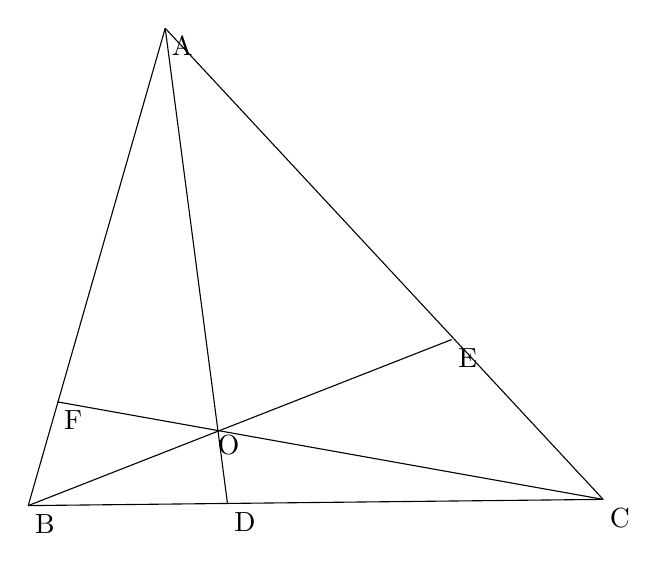
\begin{tikzpicture}[x=0.75pt,y=0.75pt,yscale=-1,xscale=1]
%uncomment if require: \path (0,300); %set diagram left start at 0, and has height of 300

%Straight Lines [id:da711612096145047] 
\draw    (211.91,30.03) -- (145.91,260.03) ;
%Straight Lines [id:da728293619031698] 
\draw    (145.91,260.03) -- (422.91,257.03) ;
%Straight Lines [id:da6290146606670881] 
\draw    (211.91,30.03) -- (422.91,257.03) ;
%Straight Lines [id:da9579416581915836] 
\draw    (211.91,30.03) -- (241.91,259.03) ;
%Straight Lines [id:da21071318124650795] 
\draw    (349.91,180.03) -- (145.91,260.03) ;
%Straight Lines [id:da20346105516117619] 
\draw    (159.91,210.03) -- (422.91,257.03) ;

% Text Node
\draw (213.91,33.03) node [anchor=north west][inner sep=0.75pt]   [align=left] {A};
% Text Node
\draw (147.91,263.03) node [anchor=north west][inner sep=0.75pt]   [align=left] {B};
% Text Node
\draw (424.91,260.03) node [anchor=north west][inner sep=0.75pt]   [align=left] {C};
% Text Node
\draw (236,225) node [anchor=north west][inner sep=0.75pt]   [align=left] {O};
% Text Node
\draw (243.91,262.03) node [anchor=north west][inner sep=0.75pt]   [align=left] {D};
% Text Node
\draw (351.91,183.03) node [anchor=north west][inner sep=0.75pt]   [align=left] {E};
% Text Node
\draw (161.91,213.03) node [anchor=north west][inner sep=0.75pt]   [align=left] {F};


\end{tikzpicture}

\vspace{200px}

\subsection{Ceva's Inverse Theorem}

Suppose we have a triangle ABC with D on BC, E on AC, F on AB, such that,
$$\frac{AF}{FB}\cdot \frac{BD}{DC} \cdot \frac{CE}{EA}=1$$
then AD,BE,CF concurrent.

\pagebreak

\section{Barycentric Coordinate}
\subsection{Definition}
The barycentric coordinates of a point can be interpreted as masses placed at the vertices of the simplex, such that the point is the center of mass (or barycenter) of these masses.



\tikzset{every picture/.style={line width=0.75pt}} %set default line width to 0.75pt        

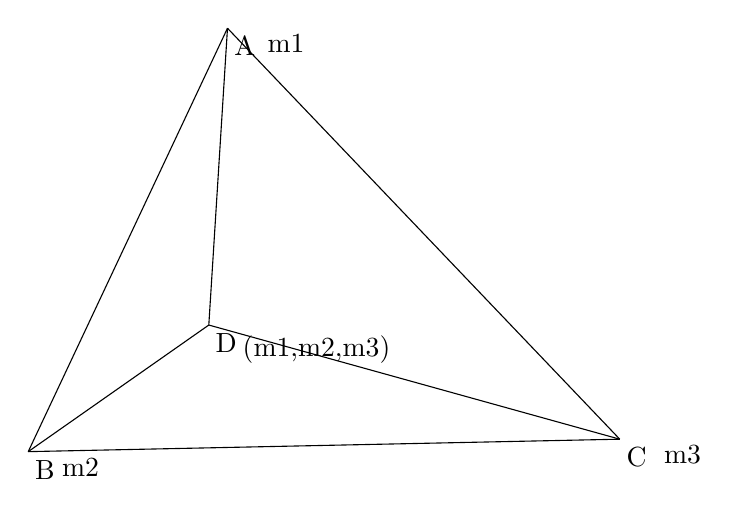
\begin{tikzpicture}[x=0.75pt,y=0.75pt,yscale=-1,xscale=1]
%uncomment if require: \path (0,300); %set diagram left start at 0, and has height of 300

%Straight Lines [id:da9034961562868877] 
\draw    (262.91,41.03) -- (166.91,245.03) ;
%Straight Lines [id:da38322702999878766] 
\draw    (451.91,239.03) -- (166.91,245.03) ;
%Straight Lines [id:da8608907326548492] 
\draw    (262.91,41.03) -- (451.91,239.03) ;
%Straight Lines [id:da9987380023335841] 
\draw    (262.91,41.03) -- (253.91,184.03) ;
%Straight Lines [id:da3386128853211863] 
\draw    (253.91,184.03) -- (166.91,245.03) ;
%Straight Lines [id:da20853567056026168] 
\draw    (253.91,184.03) -- (451.91,239.03) ;

% Text Node
\draw (264.91,44.03) node [anchor=north west][inner sep=0.75pt]   [align=left] {A};
% Text Node
\draw (168.91,248.03) node [anchor=north west][inner sep=0.75pt]   [align=left] {B};
% Text Node
\draw (453.91,242.03) node [anchor=north west][inner sep=0.75pt]   [align=left] {C};
% Text Node
\draw (255.91,187.03) node [anchor=north west][inner sep=0.75pt]   [align=left] {D};
% Text Node
\draw (281,43) node [anchor=north west][inner sep=0.75pt]   [align=left] {m1};
% Text Node
\draw (182,247) node [anchor=north west][inner sep=0.75pt]   [align=left] {m2};
% Text Node
\draw (472,241) node [anchor=north west][inner sep=0.75pt]   [align=left] {m3};
% Text Node
\draw (269,188) node [anchor=north west][inner sep=0.75pt]   [align=left] {(m1,m2,m3)};


\end{tikzpicture}


\subsection{Example}

Given BD:DC=1:2, AE:EC=1:1. Find AF:FD.

\tikzset{every picture/.style={line width=0.75pt}} %set default line width to 0.75pt        

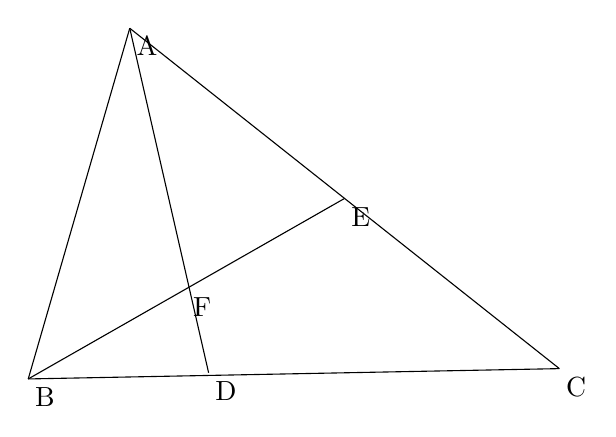
\begin{tikzpicture}[x=0.75pt,y=0.75pt,yscale=-1,xscale=1]
%uncomment if require: \path (0,300); %set diagram left start at 0, and has height of 300

%Straight Lines [id:da7675617641029677] 
\draw    (248.91,41.03) -- (200,210) ;
%Straight Lines [id:da08477900268519623] 
\draw    (248.91,41.03) -- (455.91,205.03) ;
%Straight Lines [id:da9475888247486965] 
\draw    (455.91,205.03) -- (200,210) ;
%Straight Lines [id:da019733232113179566] 
\draw    (248.91,41.03) -- (286.91,207.03) ;
%Straight Lines [id:da6042356170051348] 
\draw    (200,210) -- (352.41,123.03) ;

% Text Node
\draw (250.91,44.03) node [anchor=north west][inner sep=0.75pt]   [align=left] {A};
% Text Node
\draw (202,213) node [anchor=north west][inner sep=0.75pt]   [align=left] {B};
% Text Node
\draw (457.91,208.03) node [anchor=north west][inner sep=0.75pt]   [align=left] {C};
% Text Node
\draw (288.91,210.03) node [anchor=north west][inner sep=0.75pt]   [align=left] {D};
% Text Node
\draw (354.41,126.03) node [anchor=north west][inner sep=0.75pt]   [align=left] {E};
% Text Node
\draw (278.21,169.52) node [anchor=north west][inner sep=0.75pt]   [align=left] {F};


\end{tikzpicture}

\subsection{Problem}

Given BD:DC=1:5, AE:EC=1:4. Find AF:FD.

\tikzset{every picture/.style={line width=0.75pt}} %set default line width to 0.75pt        

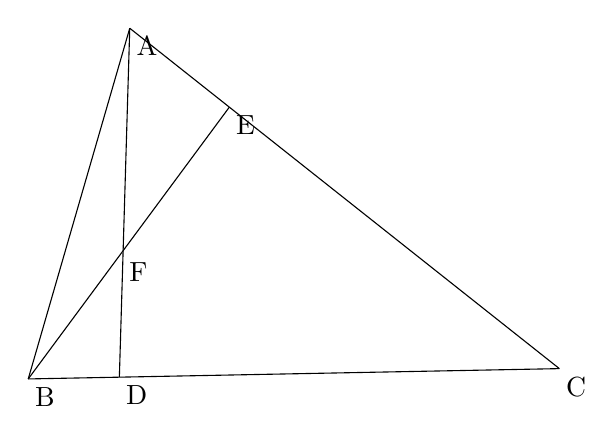
\begin{tikzpicture}[x=0.75pt,y=0.75pt,yscale=-1,xscale=1]
%uncomment if require: \path (0,300); %set diagram left start at 0, and has height of 300

%Straight Lines [id:da7675617641029677] 
\draw    (248.91,41.03) -- (200,210) ;
%Straight Lines [id:da08477900268519623] 
\draw    (248.91,41.03) -- (455.91,205.03) ;
%Straight Lines [id:da9475888247486965] 
\draw    (455.91,205.03) -- (200,210) ;
%Straight Lines [id:da019733232113179566] 
\draw    (248.91,41.03) -- (243.91,209.03) ;
%Straight Lines [id:da6042356170051348] 
\draw    (200,210) -- (296.91,79.03) ;

% Text Node
\draw (250.91,44.03) node [anchor=north west][inner sep=0.75pt]   [align=left] {A};
% Text Node
\draw (202,213) node [anchor=north west][inner sep=0.75pt]   [align=left] {B};
% Text Node
\draw (457.91,208.03) node [anchor=north west][inner sep=0.75pt]   [align=left] {C};
% Text Node
\draw (245.91,212.03) node [anchor=north west][inner sep=0.75pt]   [align=left] {D};
% Text Node
\draw (298.91,82.03) node [anchor=north west][inner sep=0.75pt]   [align=left] {E};
% Text Node
\draw (247.46,152.52) node [anchor=north west][inner sep=0.75pt]   [align=left] {F};


\end{tikzpicture}

\pagebreak

\section{Angle Bisector}


\subsection{Definition}

\vspace{30px}

\subsection{Angle Bisector  Theorem}


If AD bisects $\angle A$, then

$$\frac{BD}{CD}=\frac{AB}{AC}$$

\tikzset{every picture/.style={line width=0.75pt}} %set default line width to 0.75pt        

\begin{tikzpicture}[x=0.75pt,y=0.75pt,yscale=-1,xscale=1]
%uncomment if require: \path (0,300); %set diagram left start at 0, and has height of 300

%Straight Lines [id:da711612096145047] 
\draw    (139.91,73.03) -- (107.91,180.03) ;
%Straight Lines [id:da728293619031698] 
\draw    (107.91,180.03) -- (384.91,177.03) ;
%Straight Lines [id:da6290146606670881] 
\draw    (139.91,73.03) -- (384.91,177.03) ;
%Straight Lines [id:da9579416581915836] 
\draw    (139.91,73.03) -- (200.91,180.03) ;

% Text Node
\draw (139.91,55.03) node [anchor=north west][inner sep=0.75pt]   [align=left] {A};
% Text Node
\draw (109.91,183.03) node [anchor=north west][inner sep=0.75pt]   [align=left] {B};
% Text Node
\draw (386.91,180.03) node [anchor=north west][inner sep=0.75pt]   [align=left] {C};
% Text Node
\draw (202.91,183.03) node [anchor=north west][inner sep=0.75pt]   [align=left] {D};


\end{tikzpicture}

\vspace{100px}

\subsection{Theorem}
Angle bisectors of a trinagle are concurrent, the point is called the incenter of the triangle

\pagebreak

\subsection{Theorem}
In $\triangle ABC$ with incenter I,  $\angle BIC = 90^{\circ}+\frac{1}{2}\angle A$



\tikzset{every picture/.style={line width=0.75pt}} %set default line width to 0.75pt        

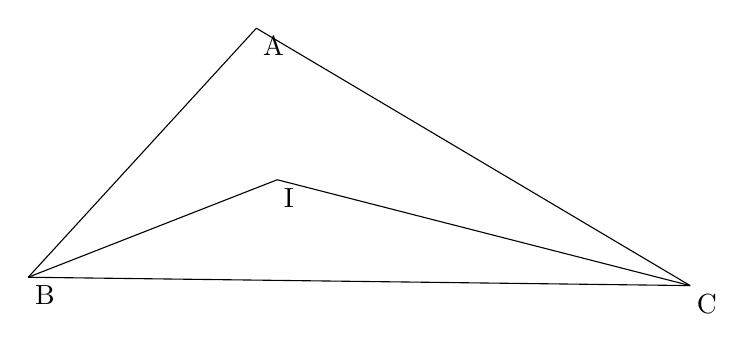
\begin{tikzpicture}[x=0.75pt,y=0.75pt,yscale=-1,xscale=1]
%uncomment if require: \path (0,300); %set diagram left start at 0, and has height of 300

%Straight Lines [id:da5905118684092199] 
\draw    (124,172) -- (442.91,176.03) ;
%Straight Lines [id:da9618382085114188] 
\draw    (124,172) -- (233.91,52.03) ;
%Straight Lines [id:da13878852480396842] 
\draw    (233.91,52.03) -- (442.91,176.03) ;
%Straight Lines [id:da09073327189026714] 
\draw    (243.96,125.03) -- (124,172) ;
%Straight Lines [id:da05856932878848253] 
\draw    (243.96,125.03) -- (442.91,176.03) ;

% Text Node
\draw (235.91,55.03) node [anchor=north west][inner sep=0.75pt]   [align=left] {A};
% Text Node
\draw (126,175) node [anchor=north west][inner sep=0.75pt]   [align=left] {B};
% Text Node
\draw (444.91,179.03) node [anchor=north west][inner sep=0.75pt]   [align=left] {C};
% Text Node
\draw (245.96,128.03) node [anchor=north west][inner sep=0.75pt]   [align=left] {I};


\end{tikzpicture}

\vspace{30px}

\subsection{Theorem}
In $\triangle ABC$ with incenter I, the circumcenter of $\triangle BIC$ is the mid point of the arc $\overset{\LARGE\frown}{BC}$.



\tikzset{every picture/.style={line width=0.75pt}} %set default line width to 0.75pt        

\begin{tikzpicture}[x=0.75pt,y=0.75pt,yscale=-1,xscale=1]
%uncomment if require: \path (0,515); %set diagram left start at 0, and has height of 515

%Straight Lines [id:da5905118684092199] 
\draw    (113,151) -- (387.96,219.03) ;
%Straight Lines [id:da9618382085114188] 
\draw    (113,151) -- (222.91,31.03) ;
%Straight Lines [id:da13878852480396842] 
\draw    (222.91,31.03) -- (387.96,219.03) ;
%Shape: Circle [id:dp8689296114246079] 
\draw   (113,168.48) .. controls (113,90.34) and (176.34,27) .. (254.48,27) .. controls (332.62,27) and (395.96,90.34) .. (395.96,168.48) .. controls (395.96,246.62) and (332.62,309.96) .. (254.48,309.96) .. controls (176.34,309.96) and (113,246.62) .. (113,168.48) -- cycle ;
%Shape: Circle [id:dp4372612009831265] 
\draw   (32.96,304.46) .. controls (32.96,200.91) and (116.91,116.96) .. (220.46,116.96) .. controls (324.01,116.96) and (407.96,200.91) .. (407.96,304.46) .. controls (407.96,408.01) and (324.01,491.96) .. (220.46,491.96) .. controls (116.91,491.96) and (32.96,408.01) .. (32.96,304.46) -- cycle ;
%Straight Lines [id:da035413888005204175] 
\draw    (113,151) -- (228.96,116.56) ;
%Straight Lines [id:da6238963393874986] 
\draw    (228.96,116.56) -- (387.96,219.03) ;

% Text Node
\draw (224.91,34.03) node [anchor=north west][inner sep=0.75pt]   [align=left] {A};
% Text Node
\draw (115,154) node [anchor=north west][inner sep=0.75pt]   [align=left] {B};
% Text Node
\draw (389.96,222.03) node [anchor=north west][inner sep=0.75pt]   [align=left] {C};
% Text Node
\draw (222.46,307.46) node [anchor=north west][inner sep=0.75pt]   [align=left] {X};
% Text Node
\draw (230.96,119.56) node [anchor=north west][inner sep=0.75pt]   [align=left] {I};


\end{tikzpicture}


\pagebreak

\section{Median}

\subsection{Definition}
\vspace{30px}

\subsection{Theorem}
Medians of triangle are concurrent. The point is called the centroid of the triangle.


\vspace{50px}

\subsection{Theorem}
In $\triangle ABC$ with centroid G and A' as the midpoint of BC, AG=2GA'.

\tikzset{every picture/.style={line width=0.75pt}} %set default line width to 0.75pt        

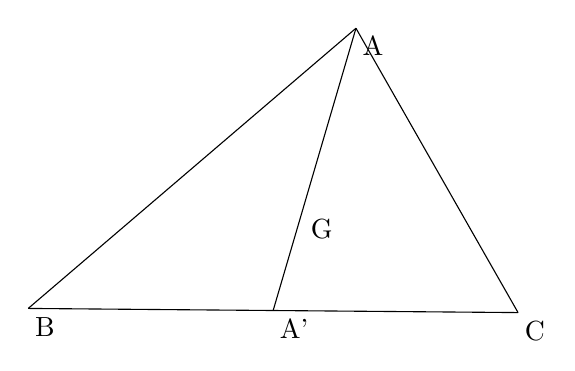
\begin{tikzpicture}[x=0.75pt,y=0.75pt,yscale=-1,xscale=1]
%uncomment if require: \path (0,389); %set diagram left start at 0, and has height of 389

%Straight Lines [id:da28332928208796315] 
\draw    (128.06,259.03) -- (364.06,261.03) ;
%Straight Lines [id:da647118791580753] 
\draw    (285.96,124.03) -- (128.06,259.03) ;
%Straight Lines [id:da4424909815278173] 
\draw    (285.96,124.03) -- (364.06,261.03) ;
%Straight Lines [id:da11044244004039627] 
\draw    (285.96,124.03) -- (246.06,260.03) ;

% Text Node
\draw (287.96,127.03) node [anchor=north west][inner sep=0.75pt]   [align=left] {A};
% Text Node
\draw (130.06,262.03) node [anchor=north west][inner sep=0.75pt]   [align=left] {B};
% Text Node
\draw (366.06,264.03) node [anchor=north west][inner sep=0.75pt]   [align=left] {C};
% Text Node
\draw (248.06,263.03) node [anchor=north west][inner sep=0.75pt]   [align=left] {A'};
% Text Node
\draw (263,215) node [anchor=north west][inner sep=0.75pt]   [align=left] {G};


\end{tikzpicture}


\vspace{50px}

\subsection{Median Length Formula}

In $\triangle ABC$ with median AA'=m, then $\frac{1}{2}m^2=b^2+c^2-\frac{1}{2}a^2$


\tikzset{every picture/.style={line width=0.75pt}} %set default line width to 0.75pt        

\begin{tikzpicture}[x=0.75pt,y=0.75pt,yscale=-1,xscale=1]
%uncomment if require: \path (0,389); %set diagram left start at 0, and has height of 389

%Straight Lines [id:da28332928208796315] 
\draw    (128.06,259.03) -- (364.06,261.03) ;
%Straight Lines [id:da647118791580753] 
\draw    (285.96,124.03) -- (128.06,259.03) ;
%Straight Lines [id:da4424909815278173] 
\draw    (285.96,124.03) -- (364.06,261.03) ;
%Straight Lines [id:da11044244004039627] 
\draw    (285.96,124.03) -- (246.06,260.03) ;

% Text Node
\draw (287.96,127.03) node [anchor=north west][inner sep=0.75pt]   [align=left] {A};
% Text Node
\draw (130.06,262.03) node [anchor=north west][inner sep=0.75pt]   [align=left] {B};
% Text Node
\draw (366.06,264.03) node [anchor=north west][inner sep=0.75pt]   [align=left] {C};
% Text Node
\draw (248.06,263.03) node [anchor=north west][inner sep=0.75pt]   [align=left] {A'};


\end{tikzpicture}

\pagebreak

\section{Height}

\subsection{Definition}
\vspace{30px}

\subsection{Theorem}

Heights of triangle are concurrent. The point is called the orthocenter of the triangle.


\tikzset{every picture/.style={line width=0.75pt}} %set default line width to 0.75pt        

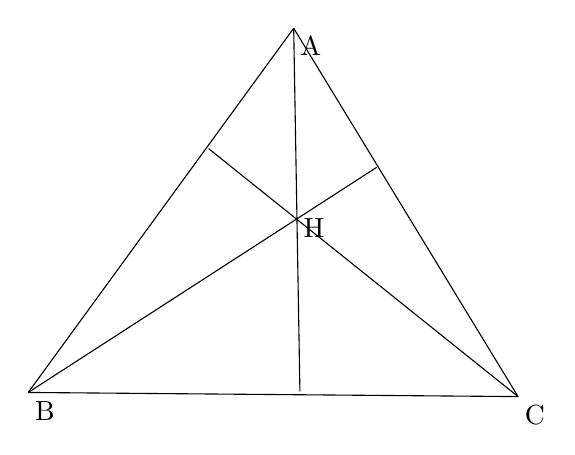
\begin{tikzpicture}[x=0.75pt,y=0.75pt,yscale=-1,xscale=1]
%uncomment if require: \path (0,389); %set diagram left start at 0, and has height of 389

%Straight Lines [id:da28332928208796315] 
\draw    (128.06,259.03) -- (364.06,261.03) ;
%Straight Lines [id:da647118791580753] 
\draw    (255.96,83.55) -- (128.06,259.03) ;
%Straight Lines [id:da4424909815278173] 
\draw    (255.96,83.55) -- (364.06,261.03) ;
%Straight Lines [id:da11044244004039627] 
\draw    (255.96,83.55) -- (258.96,258.55) ;
%Straight Lines [id:da25307184265762905] 
\draw    (295.96,150.55) -- (128.06,259.03) ;
%Straight Lines [id:da47902736207552743] 
\draw    (214.96,141.55) -- (364.06,261.03) ;

% Text Node
\draw (257.96,86.55) node [anchor=north west][inner sep=0.75pt]   [align=left] {A};
% Text Node
\draw (130.06,262.03) node [anchor=north west][inner sep=0.75pt]   [align=left] {B};
% Text Node
\draw (366.06,264.03) node [anchor=north west][inner sep=0.75pt]   [align=left] {C};
% Text Node
\draw (259.46,174.05) node [anchor=north west][inner sep=0.75pt]   [align=left] {H};


\end{tikzpicture}


\vspace{100px}

\subsection{Theorem}

In $\triangle ABC$ with orthocenter H, A' the midpoint of BC, and the circumcenter O, AH=2OA'.



\tikzset{every picture/.style={line width=0.75pt}} %set default line width to 0.75pt        

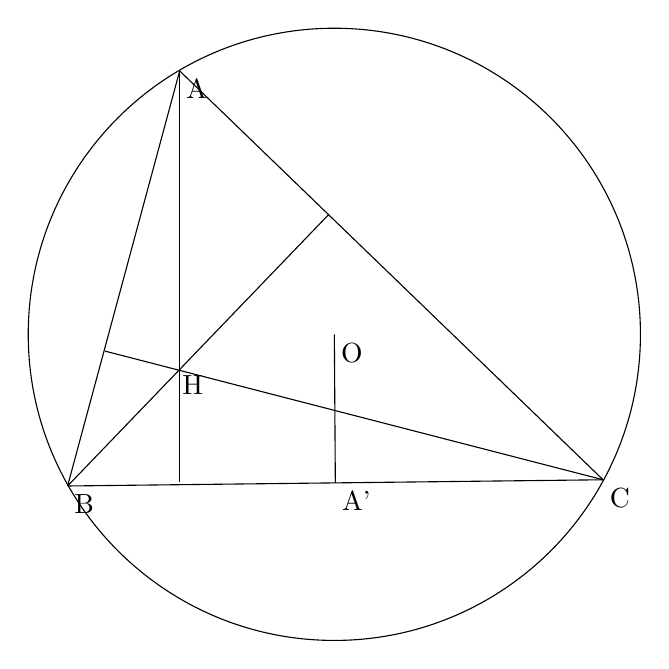
\begin{tikzpicture}[x=0.75pt,y=0.75pt,yscale=-1,xscale=1]
%uncomment if require: \path (0,389); %set diagram left start at 0, and has height of 389

%Shape: Circle [id:dp9162436210882785] 
\draw   (138,201.48) .. controls (138,120.03) and (204.03,54) .. (285.48,54) .. controls (366.93,54) and (432.96,120.03) .. (432.96,201.48) .. controls (432.96,282.93) and (366.93,348.96) .. (285.48,348.96) .. controls (204.03,348.96) and (138,282.93) .. (138,201.48) -- cycle ;
%Straight Lines [id:da7741878669053166] 
\draw    (156.96,274.55) -- (210.96,74.55) ;
%Straight Lines [id:da3851763576282945] 
\draw    (414.96,271.55) -- (156.96,274.55) ;
%Straight Lines [id:da10655267360857046] 
\draw    (210.96,74.55) -- (414.96,271.55) ;
%Straight Lines [id:da08513658544714886] 
\draw    (285.96,273.05) -- (285.48,201.48) ;
%Straight Lines [id:da351408405309773] 
\draw    (210.96,272.55) -- (210.96,74.55) ;
%Straight Lines [id:da09103761919117792] 
\draw    (282.96,143.55) -- (156.96,274.55) ;
%Straight Lines [id:da9902153949193253] 
\draw    (174.96,209.55) -- (414.96,271.55) ;

% Text Node
\draw (212.96,77.55) node [anchor=north west][inner sep=0.75pt]   [align=left] {A};
% Text Node
\draw (158.96,277.55) node [anchor=north west][inner sep=0.75pt]   [align=left] {B};
% Text Node
\draw (416.96,274.55) node [anchor=north west][inner sep=0.75pt]   [align=left] {C};
% Text Node
\draw (211,220) node [anchor=north west][inner sep=0.75pt]   [align=left] {H};
% Text Node
\draw (287.48,204.48) node [anchor=north west][inner sep=0.75pt]   [align=left] {O};
% Text Node
\draw (287.96,276.05) node [anchor=north west][inner sep=0.75pt]   [align=left] {A'};


\end{tikzpicture}

\pagebreak

\subsection{Theorem:}
O the circumcenter,G the centroid,H the orthocenter are collinear. This line is called the Euler line of the triangle.


\end{document}
